% Modified based on Xiaoming Sun's template
\documentclass{article}
\usepackage{amsmath,amsfonts,amsthm,amssymb}
\usepackage{setspace}
\usepackage{fancyhdr}
\usepackage{lastpage}
\usepackage{extramarks}
\usepackage{chngpage}
\usepackage{soul,color}
\usepackage{graphicx,float,wrapfig}

\usepackage{hyperref}
\hypersetup{
    colorlinks=true,
    linkcolor=blue,
    filecolor=magenta,      
    urlcolor=cyan,
}

\newcommand{\Class}{Mathematics for Computer Science}

% Homework Specific Information. Change it to your own
\newcommand{\Title}{Homework 3}

% In case you need to adjust margins:
\topmargin=-0.45in      %
\evensidemargin=0in     %
\oddsidemargin=0in      %
\textwidth=6.5in        %
\textheight=9.0in       %
\headsep=0.25in         %

% Setup the header and footer
\pagestyle{fancy}                                                       %
\chead{\Title}  %
\rhead{\firstxmark}                                                     %
\lfoot{\lastxmark}                                                      %
\cfoot{}                                                                %
\rfoot{Page\ \thepage\ of\ \protect\pageref{LastPage}}                          %
\renewcommand\headrulewidth{0.4pt}                                      %
\renewcommand\footrulewidth{0.4pt}                                      %

%%%%%%%%%%%%%%%%%%%%%%%%%%%%%%%%%%%%%%%%%%%%%%%%%%%%%%%%%%%%%
% Some tools
\newcommand{\enterProblemHeader}[1]{\nobreak\extramarks{#1}{#1 continued on next page\ldots}\nobreak%
                                    \nobreak\extramarks{#1 (continued)}{#1 continued on next page\ldots}\nobreak}%
\newcommand{\exitProblemHeader}[1]{\nobreak\extramarks{#1 (continued)}{#1 continued on next page\ldots}\nobreak%
                                   \nobreak\extramarks{#1}{}\nobreak}%

\newcommand{\homeworkProblemName}{}%
\newcounter{homeworkProblemCounter}%
\newenvironment{homeworkProblem}[1][Problem \arabic{homeworkProblemCounter}]%
  {\stepcounter{homeworkProblemCounter}%
   \renewcommand{\homeworkProblemName}{#1}%
   \section*{\homeworkProblemName}%
   \enterProblemHeader{\homeworkProblemName}}%
  {\exitProblemHeader{\homeworkProblemName}}%

\newcommand{\homeworkSectionName}{}%
\newlength{\homeworkSectionLabelLength}{}%
\newenvironment{homeworkSection}[1]%
  {% We put this space here to make sure we're not connected to the above.

   \renewcommand{\homeworkSectionName}{#1}%
   \settowidth{\homeworkSectionLabelLength}{\homeworkSectionName}%
   \addtolength{\homeworkSectionLabelLength}{0.25in}%
   \changetext{}{-\homeworkSectionLabelLength}{}{}{}%
   \subsection*{\homeworkSectionName}%
   \enterProblemHeader{\homeworkProblemName\ [\homeworkSectionName]}}%
  {\enterProblemHeader{\homeworkProblemName}%

   % We put the blank space above in order to make sure this margin
   % change doesn't happen too soon.
   \changetext{}{+\homeworkSectionLabelLength}{}{}{}}%

\newcommand{\Answer}{\ \\\textbf{Answer:} }
\newcommand{\Acknowledgement}[1]{\ \\{\bf Acknowledgement:} #1}

%%%%%%%%%%%%%%%%%%%%%%%%%%%%%%%%%%%%%%%%%%%%%%%%%%%%%%%%%%%%%


%%%%%%%%%%%%%%%%%%%%%%%%%%%%%%%%%%%%%%%%%%%%%%%%%%%%%%%%%%%%%
% Make title
\title{\textmd{\bf \Class: \Title}}
\date{March 18, 2019}
\author{Xingyu Su 2015010697}
%%%%%%%%%%%%%%%%%%%%%%%%%%%%%%%%%%%%%%%%%%%%%%%%%%%%%%%%%%%%%

\begin{document}
\begin{spacing}{1.1}
\maketitle \thispagestyle{empty}

%%%%%%%%%%%%%%%%%%%%%%%%%%%%%%%%%%%%%%%%%%%%%%%%%%%%%%%%%%%%%
% Begin edit from here

%%%%%%%%%%%%%%%%%%%%%%%%%%%%%%%%%%%%%%%%%%%%%%%%%%%%%%%%%%%%%
\begin{homeworkProblem}[LPV 5.4.3]

Let $A$ and $B$ be independent events. Express the probability $P(A \cup B)$ in terms of the probabilities of $A$ and $B$.

\Answer 

Because $A$ and $B$ are independent events, so $P(A \cap B) = 0$.

Then $P(A\cup B) = P(A)+P(B)-P(A\cap B)=P(A)+P(B)$

\end{homeworkProblem}
%%%%%%%%%%%%%%%%%%%%%%%%%%%%%%%%%%%%%%%%%%%%%%%%%%%%%%%%%%%%%

%%%%%%%%%%%%%%%%%%%%%%%%%%%%%%%%%%%%%%%%%%%%%%%%%%%%%%%%%%%%%
\begin{homeworkProblem}[LPV 5.4.4]

We select a subset $X$ of the set $S = \{1, 2, \dots , 100\}$ randomly and uniformly (so that every subset has the same probability of being selected). What is the probability that

(a) X has an even number of elements;

(b) both 1 and 100 belong to X;

(c) the largest element of X is 50;

(d) X has at most 2 elements.

\Answer 

(a) 
\begin{equation*}
P(a) = \frac{1}{2^{100}}\left(\binom{0}{100}+\binom{2}{100}+\cdots+\binom{98}{100}+\binom{100}{100}\right) = \frac{1}{2}
\end{equation*}

(b)
\begin{equation*}
P(b) = \frac{2^{98}}{2^{100}}=\frac{1}{4}
\end{equation*}

(c)
\begin{equation*}
P(c) = \frac{2^{49}}{2^{100}}=\frac{1}{2^{51}}\approx 4.44\times 10^{-16}
\end{equation*}

(d)
\begin{equation*}
P(d) = \frac{\binom{0}{100}+\binom{1}{100}+\binom{2}{100}}{2^{100}} \approx 4\times 10^{-27}
\end{equation*}
\end{homeworkProblem}
%%%%%%%%%%%%%%%%%%%%%%%%%%%%%%%%%%%%%%%%%%%%%%%%%%%%%%%%%%%%%


%%%%%%%%%%%%%%%%%%%%%%%%%%%%%%%%%%%%%%%%%%%%%%%%%%%%%%%%%%%%%
\begin{homeworkProblem}[LPV 5.4.5]

We flip a coin $n$ times $(n \geq 1)$. For which values of n are the following pairs of events independent?

(a) The first coin flip was heads; the number of all heads was even.

(b) The first coin flip was head; the number of all heads was more than the number of tails.

(c) The number of heads was even; the number of heads was more than the number of tails.

\Answer 

(a) To get same probability for even and odd number of all heads for left $2\sim n$ coins, $n$ should be an odd number with $n>1$. Thus, $n=3,5,7,\dots,2k+1,\dots$

(b) Since the symmetry will guarantee the probability of more heads and more tails are always the same. So any $n\geq 1$ is reasonable.

(c) To keep the symmetry, $n$ should be an even number. Thus, $n=2,4,6,\dots,2k,\dots$
\end{homeworkProblem}
%%%%%%%%%%%%%%%%%%%%%%%%%%%%%%%%%%%%%%%%%%%%%%%%%%%%%%%%%%%%%


%%%%%%%%%%%%%%%%%%%%%%%%%%%%%%%%%%%%%%%%%%%%%%%%%%%%%%%%%%%%%
\begin{homeworkProblem}[LPV 6.3.5]

Let $p$ be a prime and $1 \leq a \leq p-1$. Consider the numbers $a, 2a, 3a, \dots , (p - 1)a$. Divide each of them by $p$, to get residues $r_1 , r_2 , \dots , r_{p-1}$ . Prove that every integer from $1$ to $p-1$ occurs exactly once among these residues.

[Hint: First prove that no residue can occur twice.]

\Answer 

First prove that no residue can occur twice. Assume there are two different coefficients $k,s \ (k > s)$  that have same residues $r_k=r_s=r$. Denote the division as:
\begin{align*}
ka &= k' p+r \\
sa &= s' p+r 
\end{align*}

Then
\begin{equation*}
(k-s)a=(k'-s')p
\end{equation*}

Where $(k-s)$ and $(k'-s')$ are positive integers. But $p$ is a prime number and $0<k-s<p-1$ $1\leq a\leq p-1$ can not have factorization $p$. So there comes conflict and the Assumption is wrong.

Since there is no residue occur twice and all residues have $1\leq r_1, r_2, \dots, r_{p-1} \leq p-1$. So every integer from $1$ to $p-1$ occurs exactly once among these residues.
\end{homeworkProblem}
%%%%%%%%%%%%%%%%%%%%%%%%%%%%%%%%%%%%%%%%%%%%%%%%%%%%%%%%%%%%%


%%%%%%%%%%%%%%%%%%%%%%%%%%%%%%%%%%%%%%%%%%%%%%%%%%%%%%%%%%%%%
\begin{homeworkProblem}[LPV 6.5.2]

Consider a regular $p$-gon, and for a fixed $k (1 \leq k \leq p - 1)$, consider all $k$-subsets of the set of its vertices. Put all these $k$-subsets into a number of boxes: We put two $k$-subsets into the same box if they can be rotated into each other. For example, all $k$-subsets consisting of $k$ consecutive vertices will belong to one and the same box.

(a) Prove that if $p$ is a prime, then each box will contain exactly $p$ of these rotated copies.

(b) Show by an example that (a) does not remain true if we drop the assumption that $p$ is a prime.

(c) Use (a) to give a new proof of Lemma 6.5.2.

\Answer 

(a) Since each set can be rotated $p$ times, we just need to prove that each of the p rotated copies of a set are different. Suppose that there is a copy occurs $k$ times during the rotation. Then every other copy \textbf{must} occur $k$ times. Now we get $k|p$, and obviously $k!=p$ so $k=1$. In result, the identity is proved.

(b) Consider a case shown in Figure 1. 

\begin{figure}[htbp]
  \centering
  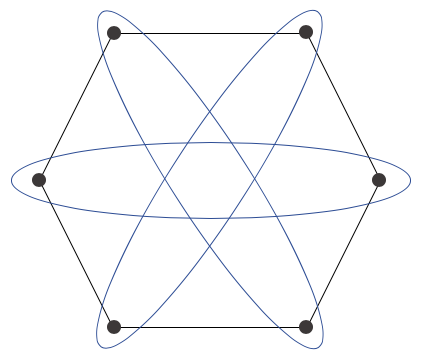
\includegraphics[width=0.3\linewidth]{figures/hw3_hexagon}
  \caption{A hexagon shows (a) is wrong when p is not a prime number}
  \label{fig:hw3_hexagon}
\end{figure}

(c) Since each box contains $p$ subsets of size $k$, the total number of subsets $\binom{p}{k}$ must satisfy $p|\binom{p}{k}$

\end{homeworkProblem}
%%%%%%%%%%%%%%%%%%%%%%%%%%%%%%%%%%%%%%%%%%%%%%%%%%%%%%%%%%%%%


%%%%%%%%%%%%%%%%%%%%%%%%%%%%%%%%%%%%%%%%%%%%%%%%%%%%%%%%%%%%%
\begin{homeworkProblem}[LPV 6.5.4]

Give a third proof of Fermat’s “Little” Theorem based on Exercise 6.3.5. 

[Hint: Consider the product $a(2a)(3a) \cdots ((p - 1)a)$]

\Answer 

From Exercise 6.3.5, we know that if $k a$ can be denote as $m_k p+r_k$ for $k=1,2,\cdots,p-1$, then every integer from $1$ to $p-1$ occurs exactly once among $r_1,r_2,\cdots,r_{p-1}$. Consider the product $a(2a)(3a) \cdots ((p - 1)a)$, we have:

\begin{equation*}
a(2a)(3a) \cdots ((p - 1)a)=(p-1)!a^{p-1}
\end{equation*}

Then:
\begin{align*}
(p-1)!(a^{p-1}-1)
  &=a(2a)(3a) \cdots ((p - 1)a)-(p-1)! \\
  &=(m_1p+r_1)(m_2p+r_2)\cdots(m_{p-1}p+r_{p-1})-r_1r_2\cdots r_{p-1} \\
  &=c_1 p^{p-1}+ c_2 p^{p-2}+\cdots+c_{p-1} p
\end{align*}
Which obviously satisfies $p|a^{p-1}-1$.
\end{homeworkProblem}
%%%%%%%%%%%%%%%%%%%%%%%%%%%%%%%%%%%%%%%%%%%%%%%%%%%%%%%%%%%%%


%%%%%%%%%%%%%%%%%%%%%%%%%%%%%%%%%%%%%%%%%%%%%%%%%%%%%%%%%%%%%
\begin{homeworkProblem}[Special Problem 1]
Alice and Bob each independently tosses an unbiased coin $n$ times. Let $X$ and $Y$ be the random variables corresponding to the number of HEADs in Alice’ and Bob’s results. Your solutions must be closed-form formulas in $n$.

(a) Determine the expected value of the random variable $X - Y$.

(b) Determine the variance of the random variable $X - Y$.

(c) Let $S$ denote the event that $X = Y$, and let $s(n) = Pr\{S\}$. Determine $s(n)$.

(d) Let $T$ denote the event that $X = Y + 1$, and let $t(n) = Pr\{T\}$. Determine $t(n)$.

\Answer 

Easy to know that $X$ and $Y$ are independent, and:
\begin{equation*}
P(X=k) = P(Y=k) = \frac{1}{2^n}\binom{n}{k}
\end{equation*}
\begin{equation*}
E(X)=E(Y)=\frac{1}{2^n}\sum_{k=0}^n k\binom{n}{k}=\frac{n}{2}
\end{equation*}
\begin{equation*}
D(X)=D(Y)=\frac{1}{2^n}\sum_{k=0}^n (k-\frac{n}{2})^2\binom{n}{k}=\frac{n}{4}
\end{equation*}

(a)
\begin{equation*}
E(X-Y) = E(X)-E(Y) = \sum_{k=0}^nk{P(X=k)-kP(Y=k)}=0
\end{equation*}

(b)
\begin{equation*}
D(X-Y) = D(X)+D(Y) = \frac{n}{2}
\end{equation*}

(c)
\begin{equation*}
s(n) = P(X=Y)
  = \sum_{k=0}^n P(X=k)P(Y=k) 
  = \frac{1}{2^{2n}}\sum_{k=0}^n \binom{n}{k}^2
\end{equation*}

\hspace{2em}
Consider equation $(1+x)^n(1+x)^n=(1+x)^{2n}$, we have:
\begin{equation*}
\left(\binom{n}{0}+x\binom{n}{1}+\cdots x^n\binom{n}{n}\right)^2=\binom{2n}{0}+x\binom{2n}{1}+\cdots x^{2n}\binom{2n}{2n}
\end{equation*}

\hspace{2em}
Compare the coefficients of $x^{n}$, we get:
\begin{align*}
\binom{2n}{n} 
  &= \binom{n}{0}\binom{n}{n}+\binom{n}{1}\binom{n}{n-1}+\cdots+\binom{n}{n}+\binom{n}{0} \\
  &= \binom{n}{0}^2+\binom{n}{1}^2+\cdots+\binom{n}{n}^2
\end{align*}

\hspace{2em}
So 
\begin{equation*}
s(n) = \frac{1}{2^{2n}}\sum_{k=0}^n \binom{n}{k}^2 = \frac{1}{2^{2n}}\binom{2n}{n}=\frac{(2n)!}{(n!)^2 2^{2n}}
\end{equation*}

(d) 
\begin{equation*}
t(n) = P(X=Y+1)
  = \sum_{k=0}^{n-1} P(X=k+1)P(Y=k)
  = \frac{1}{2^{2n}}\sum_{k=0}^{n-1} \binom{n}{k+1}\binom{n}{k}
\end{equation*}

\hspace{2em}
Similar to (c), compare the coefficients of $x^{n+1}$, we get:
\begin{align*}
\binom{2n}{n+1} 
  &= \binom{n}{n}\binom{n}{1}+\binom{n}{n-1}\binom{n}{2}+\cdots+\binom{n}{1}\binom{n}{n} \\
  &= \binom{n}{0}\binom{n}{1}+\binom{n}{1}\binom{n}{2}+\cdots+\binom{n}{n-1}\binom{n}{n}
\end{align*}

\hspace{2em}
So 
\begin{equation*}
t(n) = \frac{1}{2^{2n}}\sum_{k=0}^{n-1} \binom{n}{k}\binom{n}{k+1} = \frac{1}{2^{2n}}\binom{2n}{n+1}=\frac{(2n)!}{(n+1)!(n-1)!2^{2n}}
\end{equation*}

\end{homeworkProblem}
%%%%%%%%%%%%%%%%%%%%%%%%%%%%%%%%%%%%%%%%%%%%%%%%%%%%%%%%%%%%%


% ACKNOWLEGEMENT
\Acknowledgement

None

% End edit to here
%%%%%%%%%%%%%%%%%%%%%%%%%%%%%%%%%%%%%%%%%%%%%%%%%%%%%%%%%%%%%

\end{spacing}
\end{document}

%%%%%%%%%%%%%%%%%%%%%%%%%%%%%%%%%%%%%%%%%%%%%%%%%%%%%%%%%%%%%
